\documentclass{article}
\usepackage{graphicx}
\usepackage[utf8]{inputenc}
\usepackage[czech]{babel}
\usepackage{pdfpages}
\usepackage[margin=2.5cm]{geometry}
\usepackage{hyperref}

% Don't include subsubsections in table of contents
\setcounter{tocdepth}{2} 

\title{\textbf{Implementace překladače \\
       imperativního jazyka IFJ26}}

\date{\today}

\begin{document}

    \maketitle
    \thispagestyle{empty}

    \subsection*{Autorský tým}
        \begin{tabular}{l l l l}
            \textbf{Roman Skoupý} & 281698 & \verb|xskoupr00| & autorský podíl 25\%\\
            Matouš Jahoda & 281744 & \verb|xjahodm00| & autorský podíl  25\%\\
            Tomáš Peňás & 281746 & \verb|xpenast00| & autorský podíl  25\%\\
            Simon Šmíd & 282246 & \verb|xsmidsi00| & autorský podíl  25\%\\
        \end{tabular}
        
    \subsection*{Zvolená varianta zadání}
        Tabulka s rozptýlenými položkami s implicitním zřetězením položek (TRP-izp)
        
    \subsection*{Implementovaná rozšíření}
        \begin{itemize}
            \item FUNEXP
            \item BOOLTHEN
            \item CONTROL
            \item VALMEM
            \item ALGEBDT
            \item LAMBDAS
            \item LISTS
            \item EXTKW
            \item PARAMLISTS
        \end{itemize}
        
    \subsection*{Git repozitář se zdrojovými kódy k projektu}
        \url{https://github.com/pes50/ifj}
        

    \newpage

    
    \tableofcontents
    \thispagestyle{empty}
    

    \newpage
    
    \section{Spolupráce}
        \subsection{Rozdělení práce}
            \begin{description}
                \item[Roman Skoupý] Vedení týmu, správa repozitáře, makefile, sémantický analyzátor, \\
                převod na vnitřní kód, testy
                \item[Matouš Jahoda] Syntaktický analyzátor, testy na syntaktický analyzátor,\\
                testy na syntaktický analyzátor, revize kódu
                \item[Tomáš Peňás] Tabulka symbolů, převod na vnitřní kód, generování cíloveho kódu, \\
                testy na tabulku symbolů, revize kódu, dokumentace
                \item[Simon Šmíd] Lexikální analyzátor, vyjádření vestavěných (builtin) funkcí ve vnitřním kódu, revize kódu
            \end{description}
            
        \subsection{Způsob spolupráce}
            Na úvodní schůzce jsme si rozdělili jednotlivé komponenty a následně každý pracoval na své části. Potřebná komunikace během práce na projektu probíhala hlavně zprávami přes Discord nebo přes audio hovory na\,Discordu. Pokud se problém netýkal celého týmu, domluva často probíhala také osobně.

            Některé komponenty nebyly na začátku přiděleny a tak jsme je ve finální fázi projektu dělali společně, často přes hovor na Discordu a pomocí rozšíření Visual Studio Code "Live share"
            
            \subsubsection{Revize kódu}
                Na úvodní schůzce jsme se rozdělili do dvojic, které si navzájem měly dělat revizi kódu a potvrzovat žádosti o~začlenění do hlavní větve repozitáře. Nakonec, ale revizi prováděl ten člen týmu, který měl v dané chvíli čas a~dané komponentě alespoň trochu rozuměl. V případech že jsme na části kódu pracovali společně, vzájemně jsme svou práci kontrolovali již během psaní kódu a po dokončení jen jeden z autorů žádoost vytvořil a druhý potrvrdil.
            \subsubsection{Testování}
                Používali jsme jednotkové (kde jednotky jsou jednotlivé moduly překladače) i~integrační testy. Kromě velmi málo výjimek byly testy vygenerovány s použitím umělé inteligence. Jednotky jsme testovali až po jejich implementaci.
            \subsubsection{Formátování kódu}
                Využívali jsme formátovací styl LLVM v nástroji clang-format a pojmenovávací konvenci snake\_case.
                
    \newpage
    

    \section{Architektura překladače}
        
            \begin{figure}[h]
                \centering
                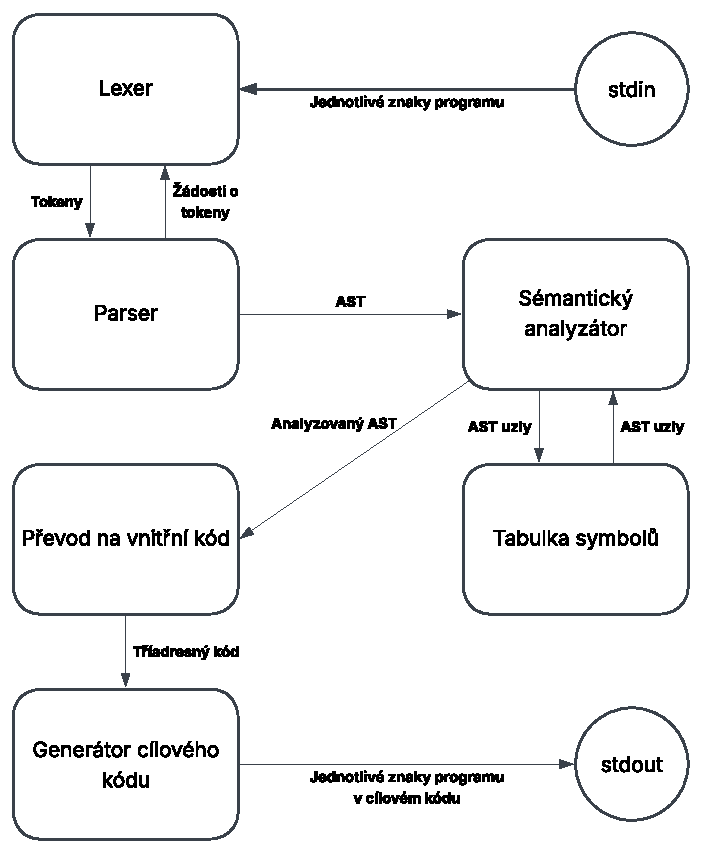
\includegraphics[scale = 1.2]{blokove_schema_ifj.pdf}
                \label{Blokové schéma překladače}
            \end{figure}
        
    
    \newpage


    \section{Popis jednotlivých modulů}
        \subsection{Lexikální analyzátor (Lexer)}
            \subsubsection{Konečný automat}
            \begin{figure}[h]
                    \centering
                    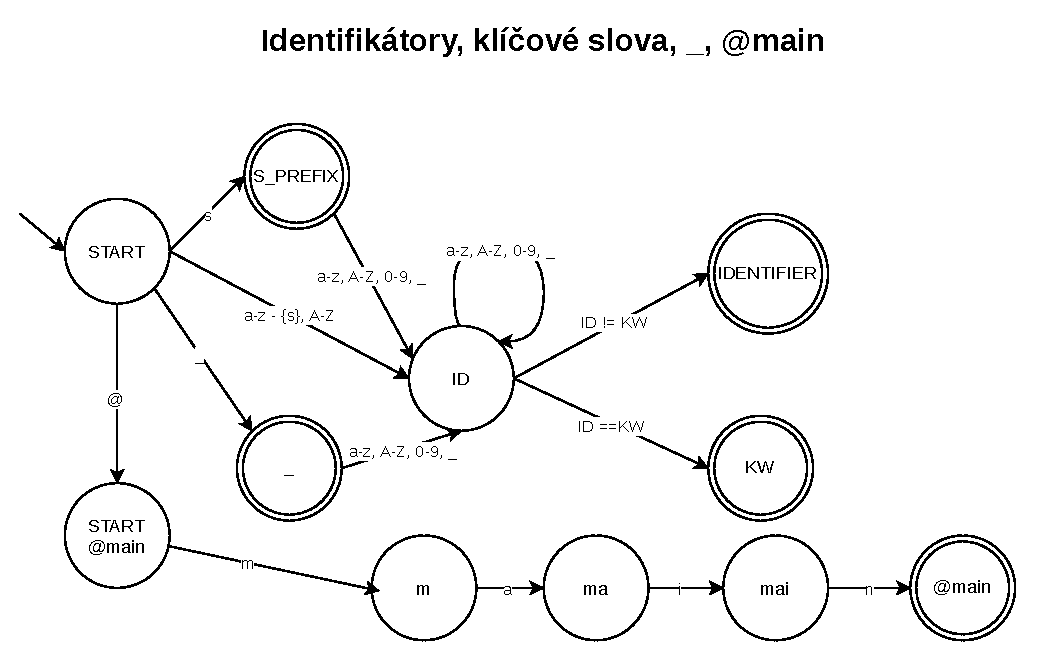
\includegraphics[scale = 1]{KA-lexer-1.pdf}
                    \label{Konečný automat pro identifikátory}
                \end{figure}
                
                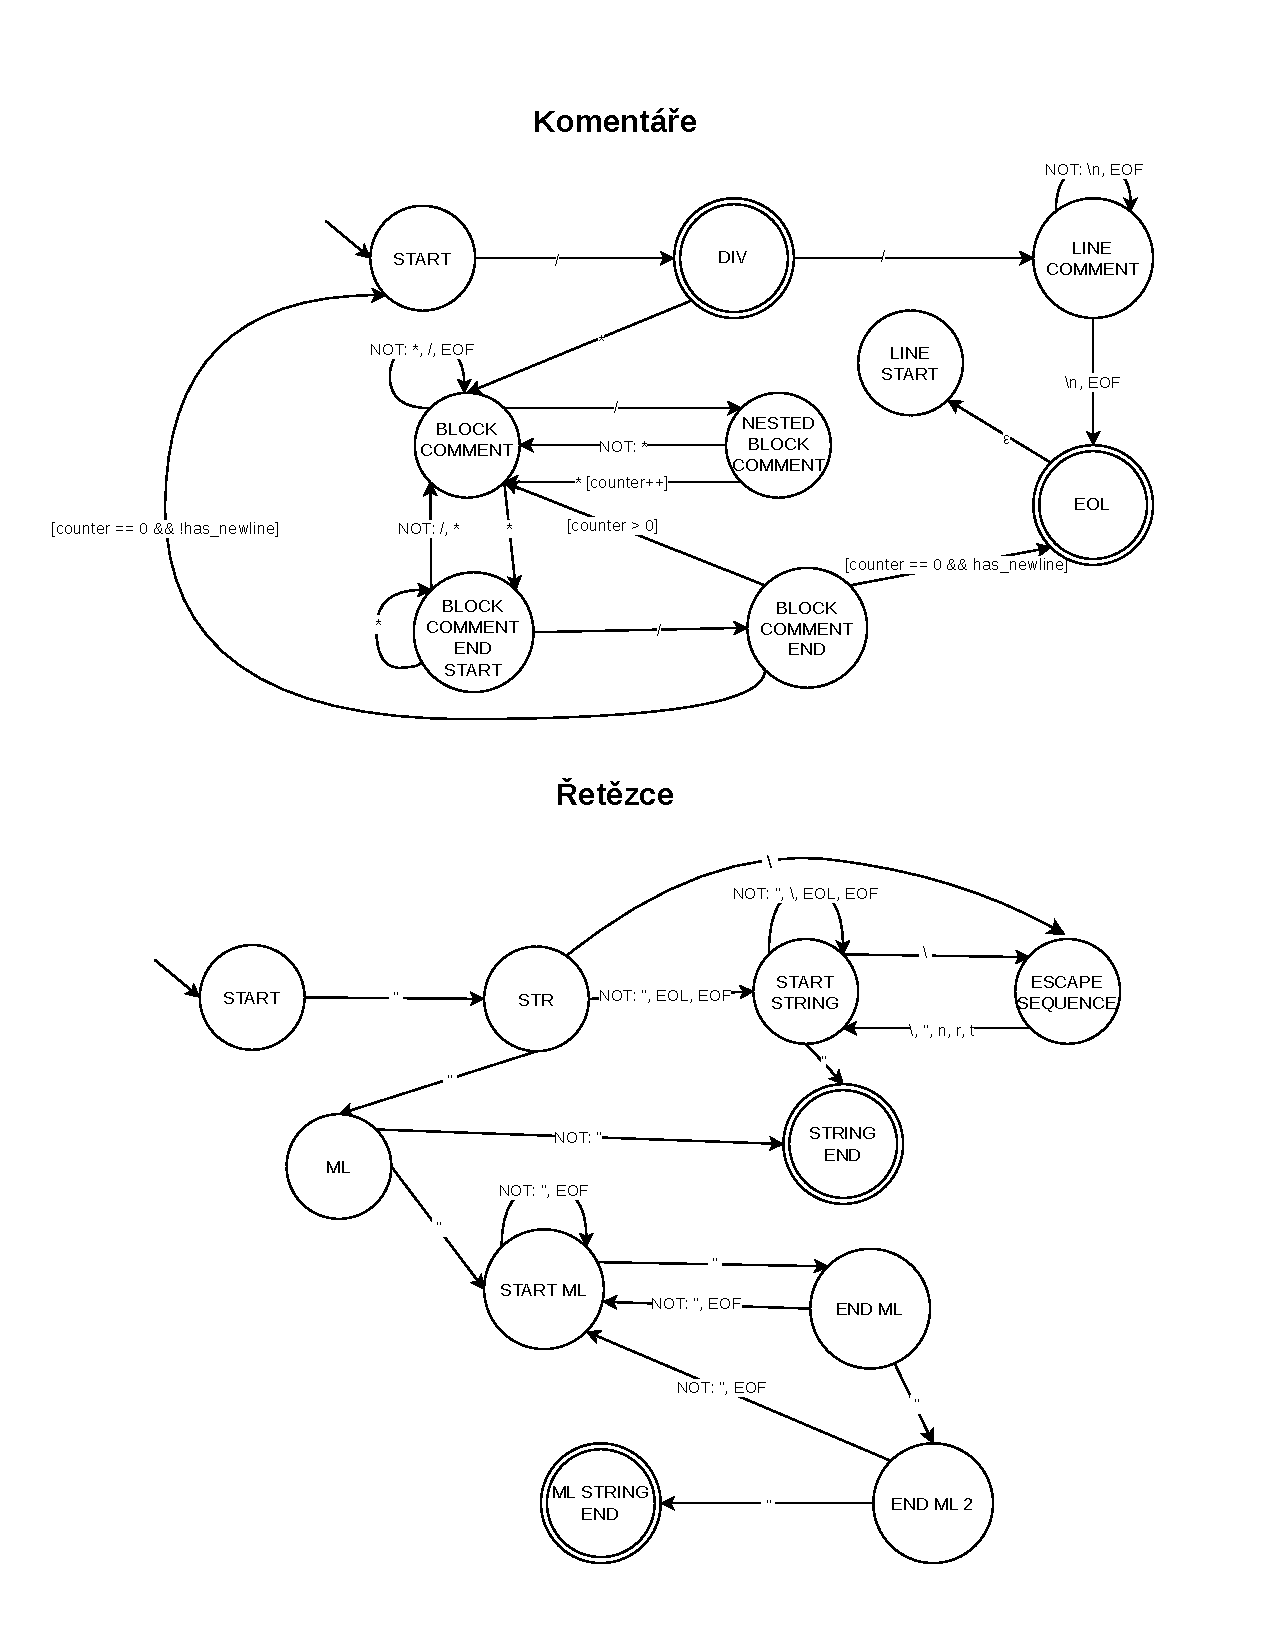
\includepdf[pages=-]{KA-lexer-2.pdf}


        \newpage


        \subsection{Syntaktický analyzátor (Parser)}
            \subsubsection{LL gramatika}
            \subsubsection{Precedenční tabulka}

        \subsection{Sémantický analyzátor}
            
        \subsection{Tabulka symbolů}
            V tabulce jsme pro rozptylování položek využili Fowler–Noll–Vo hašovací algoritmus pro 32bitové hašování, konkrétně jeho variantu FNV-1a \cite{FNV-1a} %TODO

        \subsection{Převod na vnitřní kód}
            
        \subsection{Generátor cílového kódu}
            

    \newpage


    \section{Využití AI}
        

    \newpage

    
    \addcontentsline{toc}{section}{Převzaté zdroje}
    \def \refname {Převzaté zdroje}
    \begin{thebibliography}{99}
        \bibitem{FNV-1a} L. Noll, K. Vo, D. Eastlake 3rd, and T. Hansen, "The FNV Non-Cryptographic Hash Algorithm," RFC 9923, Feb. 2026. [Online].\\
        Available: \mbox{\url{https://www.rfc-editor.org/info/rfc9923}}
        %TODO IDK jestli jsme prevzali jeste neco
    \end{thebibliography}
\end{document}